\documentclass[UTF8,a4paper,zihao=-4]{ctexart}
\usepackage[margin=22mm]{geometry}
\usepackage{amsmath,amssymb,graphicx,enumitem,booktabs,array}
\usepackage[hidelinks]{hyperref}
\usepackage{caption}
\captionsetup{font=small,labelsep=quad}
\ctexset{section={name={第,章},number=\chinese{section},format=\Large\bfseries},
subsection={number=\arabic{section}.\arabic{subsection},format=\large\bfseries}}
\numberwithin{equation}{section}
\numberwithin{figure}{section}
\numberwithin{table}{section}
\renewcommand{\theequation}{\arabic{section}.\arabic{equation}}
\renewcommand{\thefigure}{\arabic{section}-\arabic{figure}}
\renewcommand{\thetable}{\arabic{section}-\arabic{table}}
\setlength{\parindent}{2em}
\setlength{\parskip}{2pt}
\begin{document}
\begin{center}{\LARGE\bfseries 面向三种硬件场景的神经网络多核切图与协同调度研究\par}\end{center}
\vspace{1em}
\section{问题重述}
\subsection{问题背景}
神经网络计算图由相互依赖的计算操作和中间张量构成。将计算图部署到多核处理器时，操作如何切分、分配到哪些核心以及各核心按什么顺序执行，会共同影响执行时间和数据搬运量。矩阵与向量操作的工作特征不同，核心间传输还会消耗同步和带宽资源；有限的片上存储则可能引发换入换出。因此，调度方案需要根据计算图结构和硬件执行规则联合确定。

本题设置了三个执行场景：问题一将子图作为独立任务，问题二允许同核子图合并执行，问题三在问题二基础上启用共享 FIFO 缓存。三个场景具有不同的任务边界、通信开销和数据复用方式，需要分别建立目标与约束。

\subsection{问题重述}
\textbf{问题一：独立子图任务下的切图与调度。}给定计算图、核心数及硬件配置，将操作划分为子图，为子图分配核心并确定各核心上的执行顺序。每个子图对应一个独立 Task。Task 间等待依赖前驱所在核心：题面规定核内等待为 100 cycles、跨核等待为 1000 cycles；同一核心上相邻 Task 的边界数据也按题目规则处理。要求在满足依赖、Task 顺序和存储规则的前提下缩短全图完成时间。

\textbf{问题二：同核 Task 合并下的通信协同调度。}在问题一的计算图及核心分配框架上，将同一核心上的子图合并为一个 Task。跨核依赖需要经过 COPY\_OUT、同步和 COPY\_IN，跨核同步延迟为 500 cycles。同核数据可在片上复用。模型需在核间并行收益、跨核通信、Pipe 负载均衡和片上存储压力之间进行权衡。

\textbf{问题三：启用共享 FIFO L2 缓存的调度。}沿用问题二的同核 Task 合并与跨核通信规则，增加共享只读 FIFO L2 缓存。L2 容量为 1 MiB、带宽为 250 B/cycle；DDR 为共享 60 B/cycle，Cache 初始为空。模型需考虑请求发射次序、未命中读取完成后的插入和 FIFO 淘汰对命中结果的影响，并比较 Cache 对 DDR 流量与总完成时间的作用。

三个场景共用的片上容量为 L1=524,288 B、UB=131,072 B。容量约束和带宽约束分别描述数据驻留和搬运速率，应独立处理。

\section{问题分析}
\subsection{问题一的分析}
问题一中，一个子图就是一个 Task。切分粒度会影响 Task 数量、Task 等待和边界张量处理，也决定操作能否分散到多个核心并行执行。弱连通分量内部没有跨分量依赖，可作为初始装箱单元；但若一个连通分量占据大部分操作或计算周期，单纯按分量分配会限制并行度，需要进一步考察合法的拓扑切分。

对当前问题一冻结求解器，结构方法包括双 Pipe 分量装箱、依据图深度/汇合/共享关系切分、按就绪 Task 贪心分配核心及有界合并。求解过程使用固定策略，不在单个输入上调用官方评估器挑选候选。调度分析至少需要考虑每核矩阵和向量工作量、依赖关键路径、Task 激活、DDR 搬运与片上容量。总计算量均分不能反映不同 Pipe 的负载差异；各依赖等待也可能重叠，不能简单累加为实际完成时间。

\subsection{问题二的分析}
问题二将同核子图合并为一个 Task，核内数据复用更直接，但跨核依赖需承担 COPY 与同步代价。若为减少通信而把相关操作集中到一核，可能出现矩阵或向量 Pipe 过载；若将计算分散到更多核心，又可能增加跨核搬运并占用共享 DDR 带宽。

当前问题二模型以双 Pipe 负载、跨核关键路径、DDR 流量和静态张量存活压力构造候选排序代理，并从有限的分量装箱、深度带和数据感知切分方案中选择。静态内存压力不等同官方 Step 2 的准确 spill 量；正式 makespan、实际搬运及容量行为仍以冻结方案后的官方执行为准。开发阶段对风险系数进行全局标定，不能把在给定 100 图上取得的结果解释为分布外保证。

\subsection{问题三的分析}
问题三在问题二基础上引入 FIFO 缓存。张量是否命中，取决于读请求发生时张量是否已完成读取并插入缓存，以及此前插入的数据是否已将其淘汰。命中不刷新 FIFO 顺序，超过容量的张量不能驻留。因此，单独统计复用次数无法判断实际命中。

当前问题三冻结版本依据输入图构造有限种结构方案，并用自身的事件与驻留模型排序；每次推理不调用官方评估器或读取历史解。开发诊断使用过给定图集的官方反馈，故需将“单次推理不调用评估器”与“全局开发未使用评分标签”区分。缓存命中能减少 DDR 读取，但命中流量仍占用 L2 带宽。缓存收益应在同一冻结方案下配对比较，以避免把切图差异误认为缓存收益。

\subsection{统一的多目标设计}
令方案为 $\pi$，问题编号为 $q\in\{1,2,3\}$。在结构合法且满足片上存储约束的方案集合内，分别考虑：

\begin{equation*}
\min \mathbf f_1(\pi)=
\bigl(T_1(\pi),\ Q_1(\pi),\ I_{\mathrm{imb},1}(\pi)\bigr),
\end{equation*}
\begin{equation*}
\min \mathbf f_2(\pi)=
\bigl(T_2(\pi),\ Q_{\mathrm{cross},2}(\pi),\ I_{\mathrm{imb},2}(\pi)\bigr),
\end{equation*}
\begin{equation*}
\min \mathbf f_3(\pi)=
\bigl(T_3(\pi),\ Q_{\mathrm{DDR},3}(\pi),\ -Q_{\mathrm{hit},3}(\pi),\ I_{\mathrm{imb},3}(\pi)\bigr).
\end{equation*}
其中，$T_q$ 为全图完成时间，$Q_q$ 表示场景相应的新增通信或 DDR 字节，$Q_{\mathrm{hit},3}$ 为 FIFO 命中字节，$I_{\mathrm{imb},q}$ 为核心/Pipe 工作量不均衡度。存储容量作为硬约束单独检查，不再作为目标重复惩罚；问题三的 1 MiB FIFO 容量由题设缓存插入与淘汰规则保证。真实时间、换入换出量和缓存命中以官方执行程序为准；搜索阶段若使用估计量，须明确标为代理值。

令 $x_{vk}\in\{0,1\}$ 表示操作 $v$ 是否分配到核心 $k$，$r_v$ 表示其合法拓扑执行序位。基本结构约束为：

\begin{equation*}
\sum_{k=0}^{n-1}x_{vk}=1\quad(\forall v\in V),\qquad
r_u<r_v\quad(\forall (u,v)\in E).
\end{equation*}
此外还需保证每个子图唯一分核、每核子图序列合法，且原始依赖与同核顺序联合后无环。

对每个核心 $k$，理想内存可行性约束为：

\begin{equation*}
H_{k,\mathrm{L1}}(\pi)\le 524288,\qquad
H_{k,\mathrm{UB}}(\pi)\le 131072.
\end{equation*}
DDR/L2 带宽可导出完成时间下界：

\begin{equation*}
T_q(\pi)\ge
\max\left\{
\max_{k,p}W_{kp}(\pi),\
L_{\mathrm{dep},q}(\pi),\
\frac{Q_{D,q}^{\min}(\pi)}{60},\
\mathbf 1_{q=3}\frac{Q_{L,q}^{\min}(\pi)}{250}
\right\}.
\end{equation*}
该式给出资源和依赖下界，不是精确 makespan 的可加公式。多个资源可能并行工作，最终时间应由官方离散事件模拟决定。方案 $\pi_a$ 支配 $\pi_b$，是指所有待最小化指标均不劣且至少一项严格更优。透明的决策流程是先筛除结构和内存不可行方案，再保留 Pareto 非支配解，最后使用预先固定且仅依赖输入图与硬件参数的规则输出单一方案。

\section{模型假设}
1. \textbf{计算图假设。}输入操作与张量依赖构成有向无环图；操作周期、执行 Pipe、张量大小和存储位置按官方数据读取。

2. \textbf{分配唯一性假设。}每个操作被且仅被分配到一个子图；每个子图被且仅被分配到一个核心。

3. \textbf{执行顺序假设。}方案满足原始依赖，以及题目规定的 Task 依赖和核心内子图顺序。只施加题目实际要求的有向无环约束。

4. \textbf{资源容量假设。}L1 和 UB 是分别受限的片上资源，不能将两者容量合并后判断可行。

5. \textbf{共享带宽假设。}DDR 与问题三中的 L2 按题设作为共享带宽池；带宽下界不等同实际执行时长。

6. \textbf{FIFO 假设。}问题三缓存按题目 FIFO 查询、插入与淘汰规则工作；不假设题目未规定的预取或预热行为。

7. \textbf{描述统计假设。}第五章仅汇总官方 100 个原始输入图的结构和规模特征，不将评估器输出混入输入统计。

8. \textbf{近似量边界。}逻辑生命周期峰值、预测命中和资源时间下界用于分析或候选排序，不宣称它们等于官方执行器测得的峰值、命中或 makespan。

9. \textbf{评估器边界。}当前单次推理不调用官方评估器；开发标定可能使用评分反馈，二者在方法叙述和结果解释中分别说明。

\section{符号说明}
\begin{table}[htbp]
\centering\small
\begin{tabular}{lrr}
\toprule
符号 & 含义 & 单位/范围 \\
\midrule
$G=(V\cup\mathcal T,E)$ & 操作、张量和依赖边组成的计算图 & — \\
$V,\mathcal T,E$ & 操作、张量、依赖边集合 & — \\
$d_v$ & 操作 $v$ 的计算周期 & cycles \\
$p(v)$ & 操作 $v$ 使用的 Pipe 类型 & 矩阵/向量等 \\
$b_t$ & 张量 $t$ 的大小 & B \\
$\operatorname{pos}(t)$ & 张量 $t$ 的存储层级 & L1/UB \\
$n,k$ & 核心数和核心索引 & $k=0,\ldots,n-1$ \\
$\phi(v)$ & 操作到子图的映射 & — \\
$\kappa(s)$ & 子图 $s$ 到核心的映射 & — \\
$\pi_k$ & 核心 $k$ 上子图的执行序列 & — \\
$\tau_q(v)$ & 场景 $q$ 中操作对应的 Task & — \\
$W_{kp}$ & 核心 $k$ 上 Pipe $p$ 的总工作量 & cycles \\
$Q_q$ & 场景 $q$ 的相关搬运字节量 & B \\
$H_{k,m}$ & 核心 $k$ 在存储层级 $m$ 的峰值占用 & B \\
$C_m$ & 存储层级 $m$ 的容量 & B \\
$B_D,B_L$ & DDR、L2 带宽 & B/cycle \\
$C_L$ & L2 容量 & B \\
$T_q(\pi)$ & 官方执行器下方案 $\pi$ 的完成时间 & cycles \\
$L_{\mathrm{dep},q}$ & 依赖与场景同步形成的关键路径下界 & cycles \\
$I_{\mathrm{imb},q}$ & 核心/Pipe 工作量不均衡度 & 无量纲 \\
$Q_{\mathrm{hit},3}$ & 问题三中的 L2 命中字节数 & B \\
\bottomrule
\end{tabular}
\end{table}
\section{描述性统计}
\subsection{数据来源与预处理}
统计对象为官方输入目录中的 100 个计算图。处理过程保留原始操作周期、张量字节数、图边和案例编号，并从原图计算操作数、DAG 边数、弱连通分量数、最大分量占比、矩阵/向量周期、关键路径、张量总字节及共享外部输入等特征。输入文件 SHA256 和 7 项基础 profile 均与项目清单逐图核对，100/100 匹配。

规模特征的原始值保留在 CSV 与统计 JSON 中；为了显示不同数量级，绘图时对长尾计数使用对数坐标，不对数据做截尾或 winsorize。比例变量保留在 $[0,1]$。本章仅分析输入特征，不读取完成时间、加速比、spill 或 Cache 评估输出。

\subsection{数据规模与计算特征}
表 5-1 中每项依次给出最小值、第一四分位数、中位数、均值、第三四分位数和最大值。

\begin{center}\textbf{表 5-1  100 个输入图的规模和计算特征}\end{center}
\begin{table}[htbp]
\centering\small
\begin{tabular}{lrrrrrr}
\toprule
特征 & min & Q1 & 中位数 & 均值 & Q3 & max \\
\midrule
计算操作数 & 552 & 1,110.75 & 3,720.5 & 6,345.06 & 7,096 & 35,705 \\
DAG 边数 & 400 & 1,266.25 & 4,017 & 7,406.41 & 8,269.75 & 38,493 \\
总计算周期 & 23,052 & 162,732.75 & 509,952 & 3,179,741.84 & 1,848,864 & 61,275,840 \\
关键路径周期 & 400 & 2,500.5 & 6,140 & 39,921.77 & 24,796.5 & 863,040 \\
矩阵 Pipe 周期 & 0 & 63,177 & 256,920 & 2,728,477.23 & 1,345,339 & 58,915,232 \\
向量 Pipe 周期 & 9,988 & 58,334 & 144,314.5 & 451,264.61 & 347,998.5 & 7,714,975 \\
$W/S$ 并行度代理 & 3.42 & 20.20 & 43.13 & 416.22 & 305.17 & 6,258.78 \\
\bottomrule
\end{tabular}
\end{table}
总计算周期的均值约为 318 万 cycles，中位数约为 51 万 cycles，说明少数大图显著拉高均值。$W/S$ 定义为总操作工作量与计算关键路径之比，仅表示图结构提供的并行空间，不是可实现的加速比。

\begin{figure}[htbp]
\centering
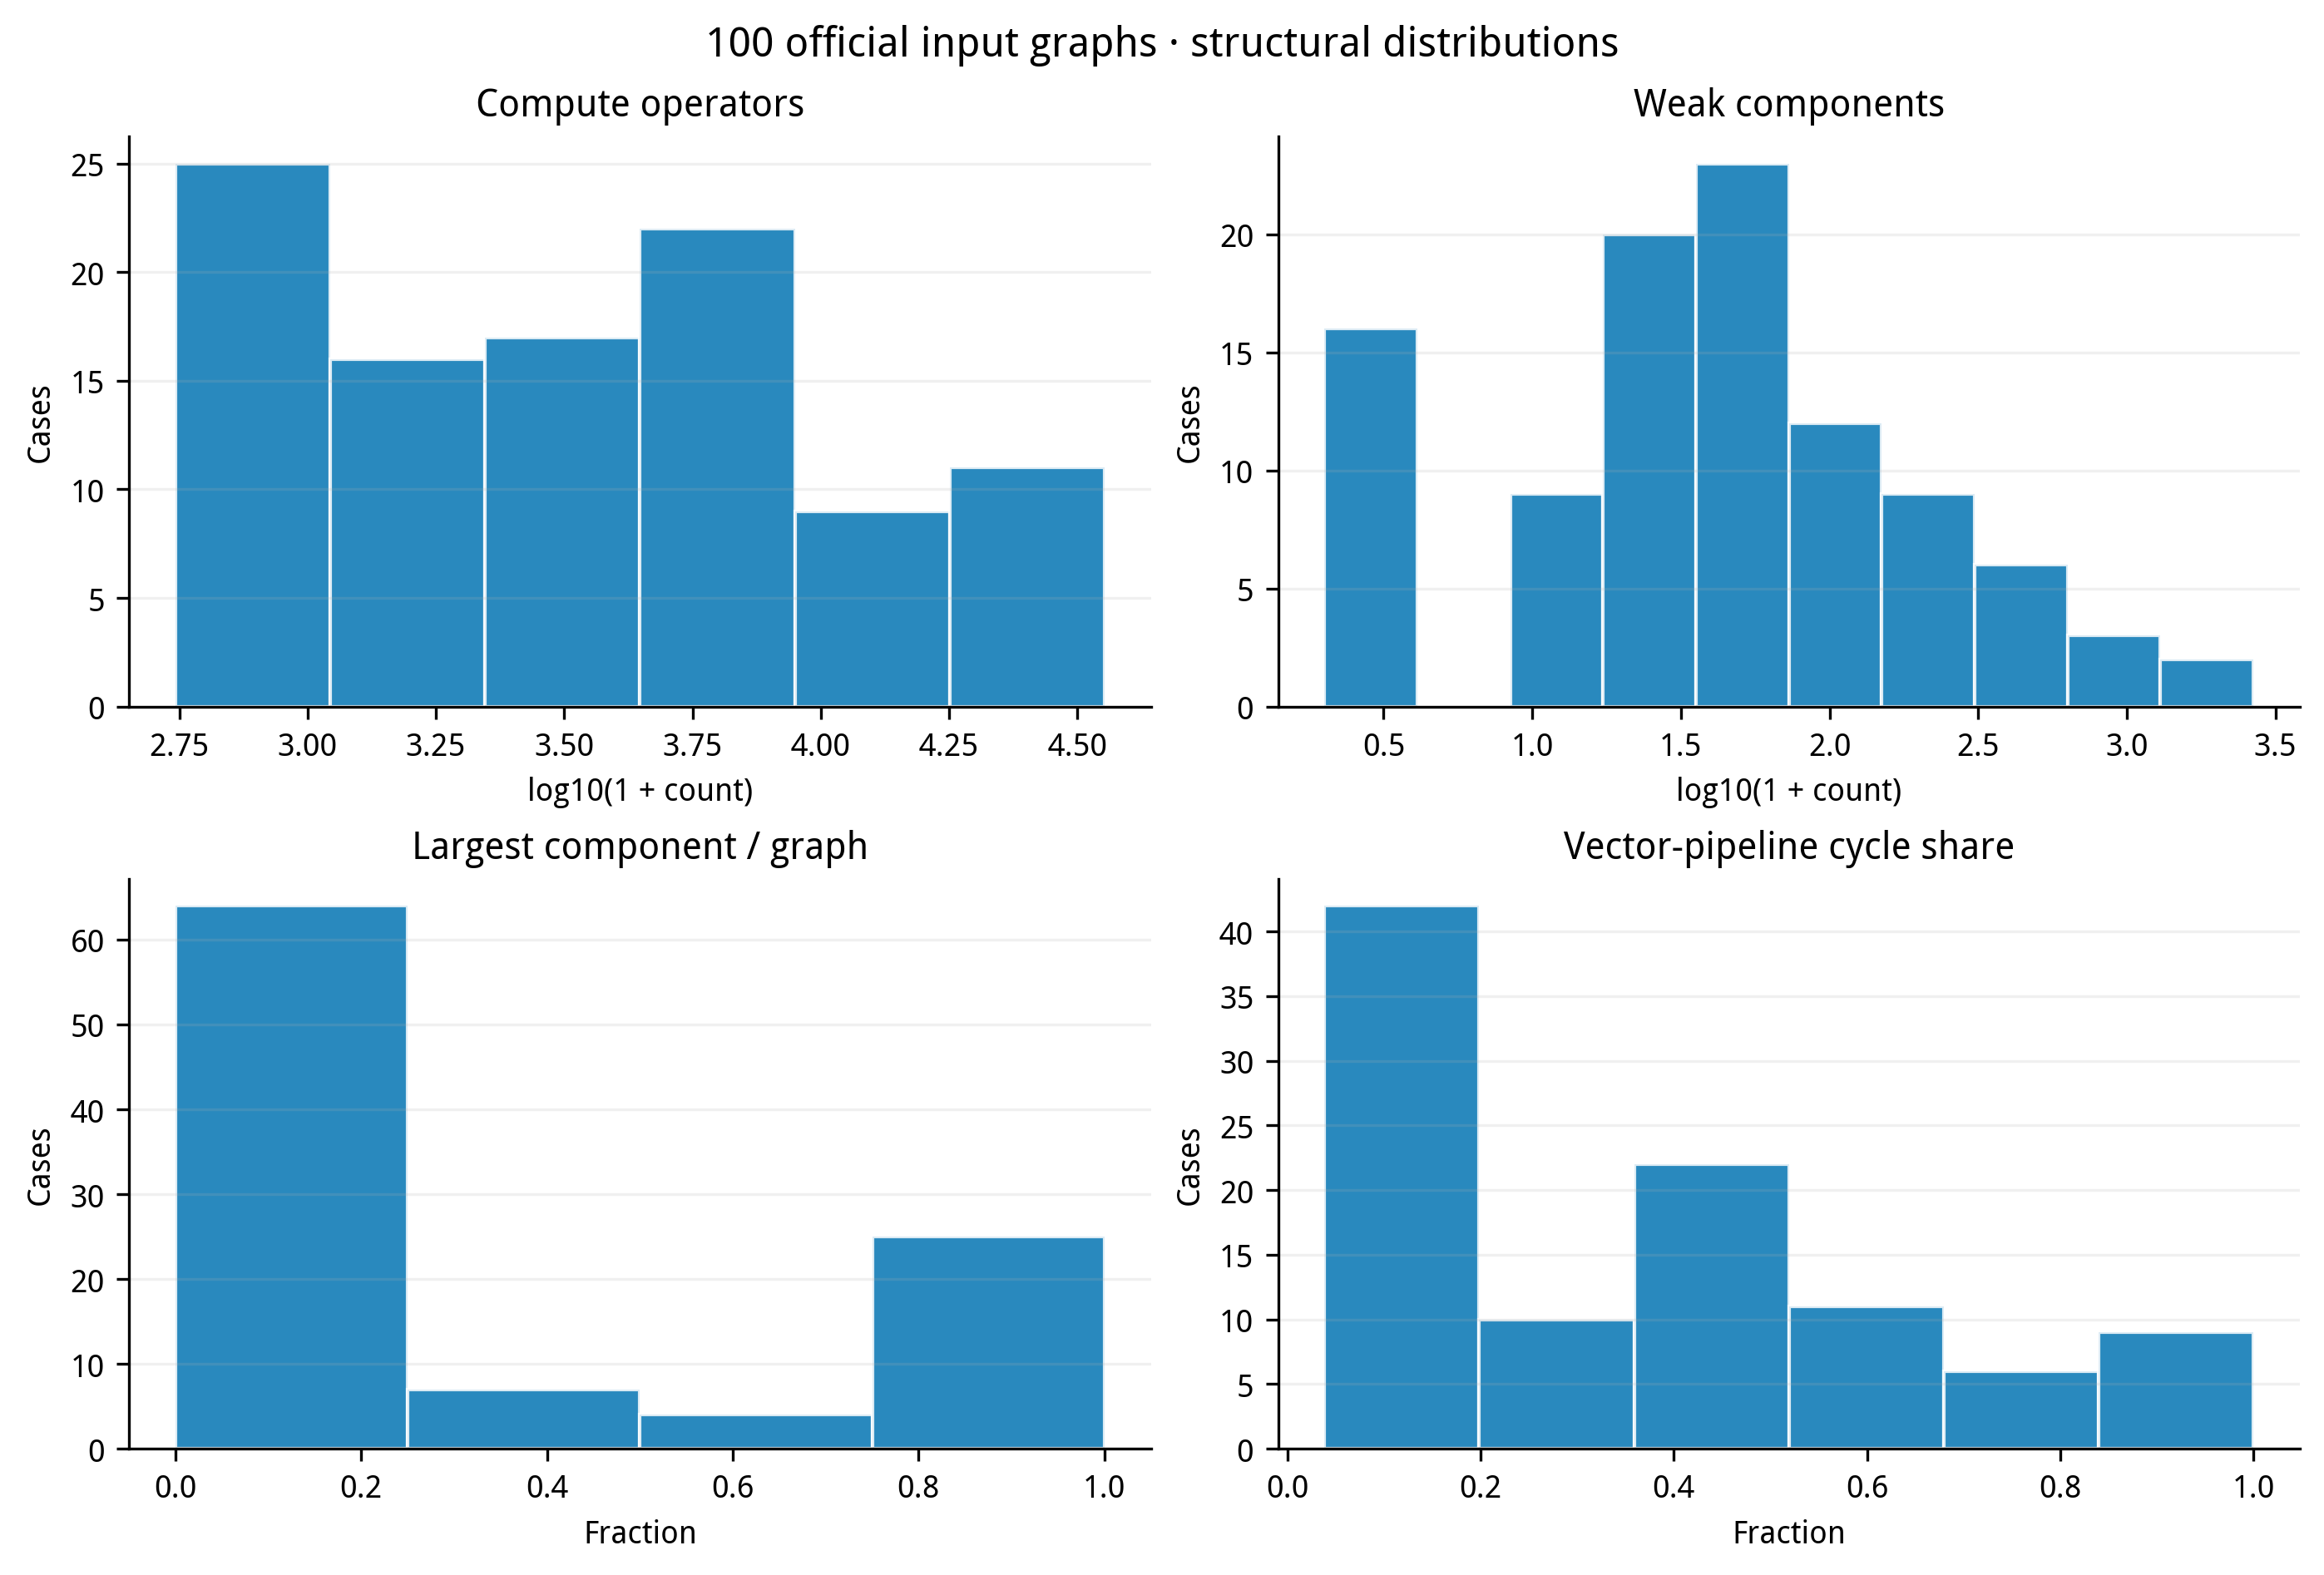
\includegraphics[width=0.88\linewidth]{../all_questions_fresh_v3/figures/fig01_input_distributions.png}
\caption{计算操作数、分量数、最大分量占比和向量 Pipe 占比的分布}
\end{figure}
\begin{figure}[htbp]
\centering
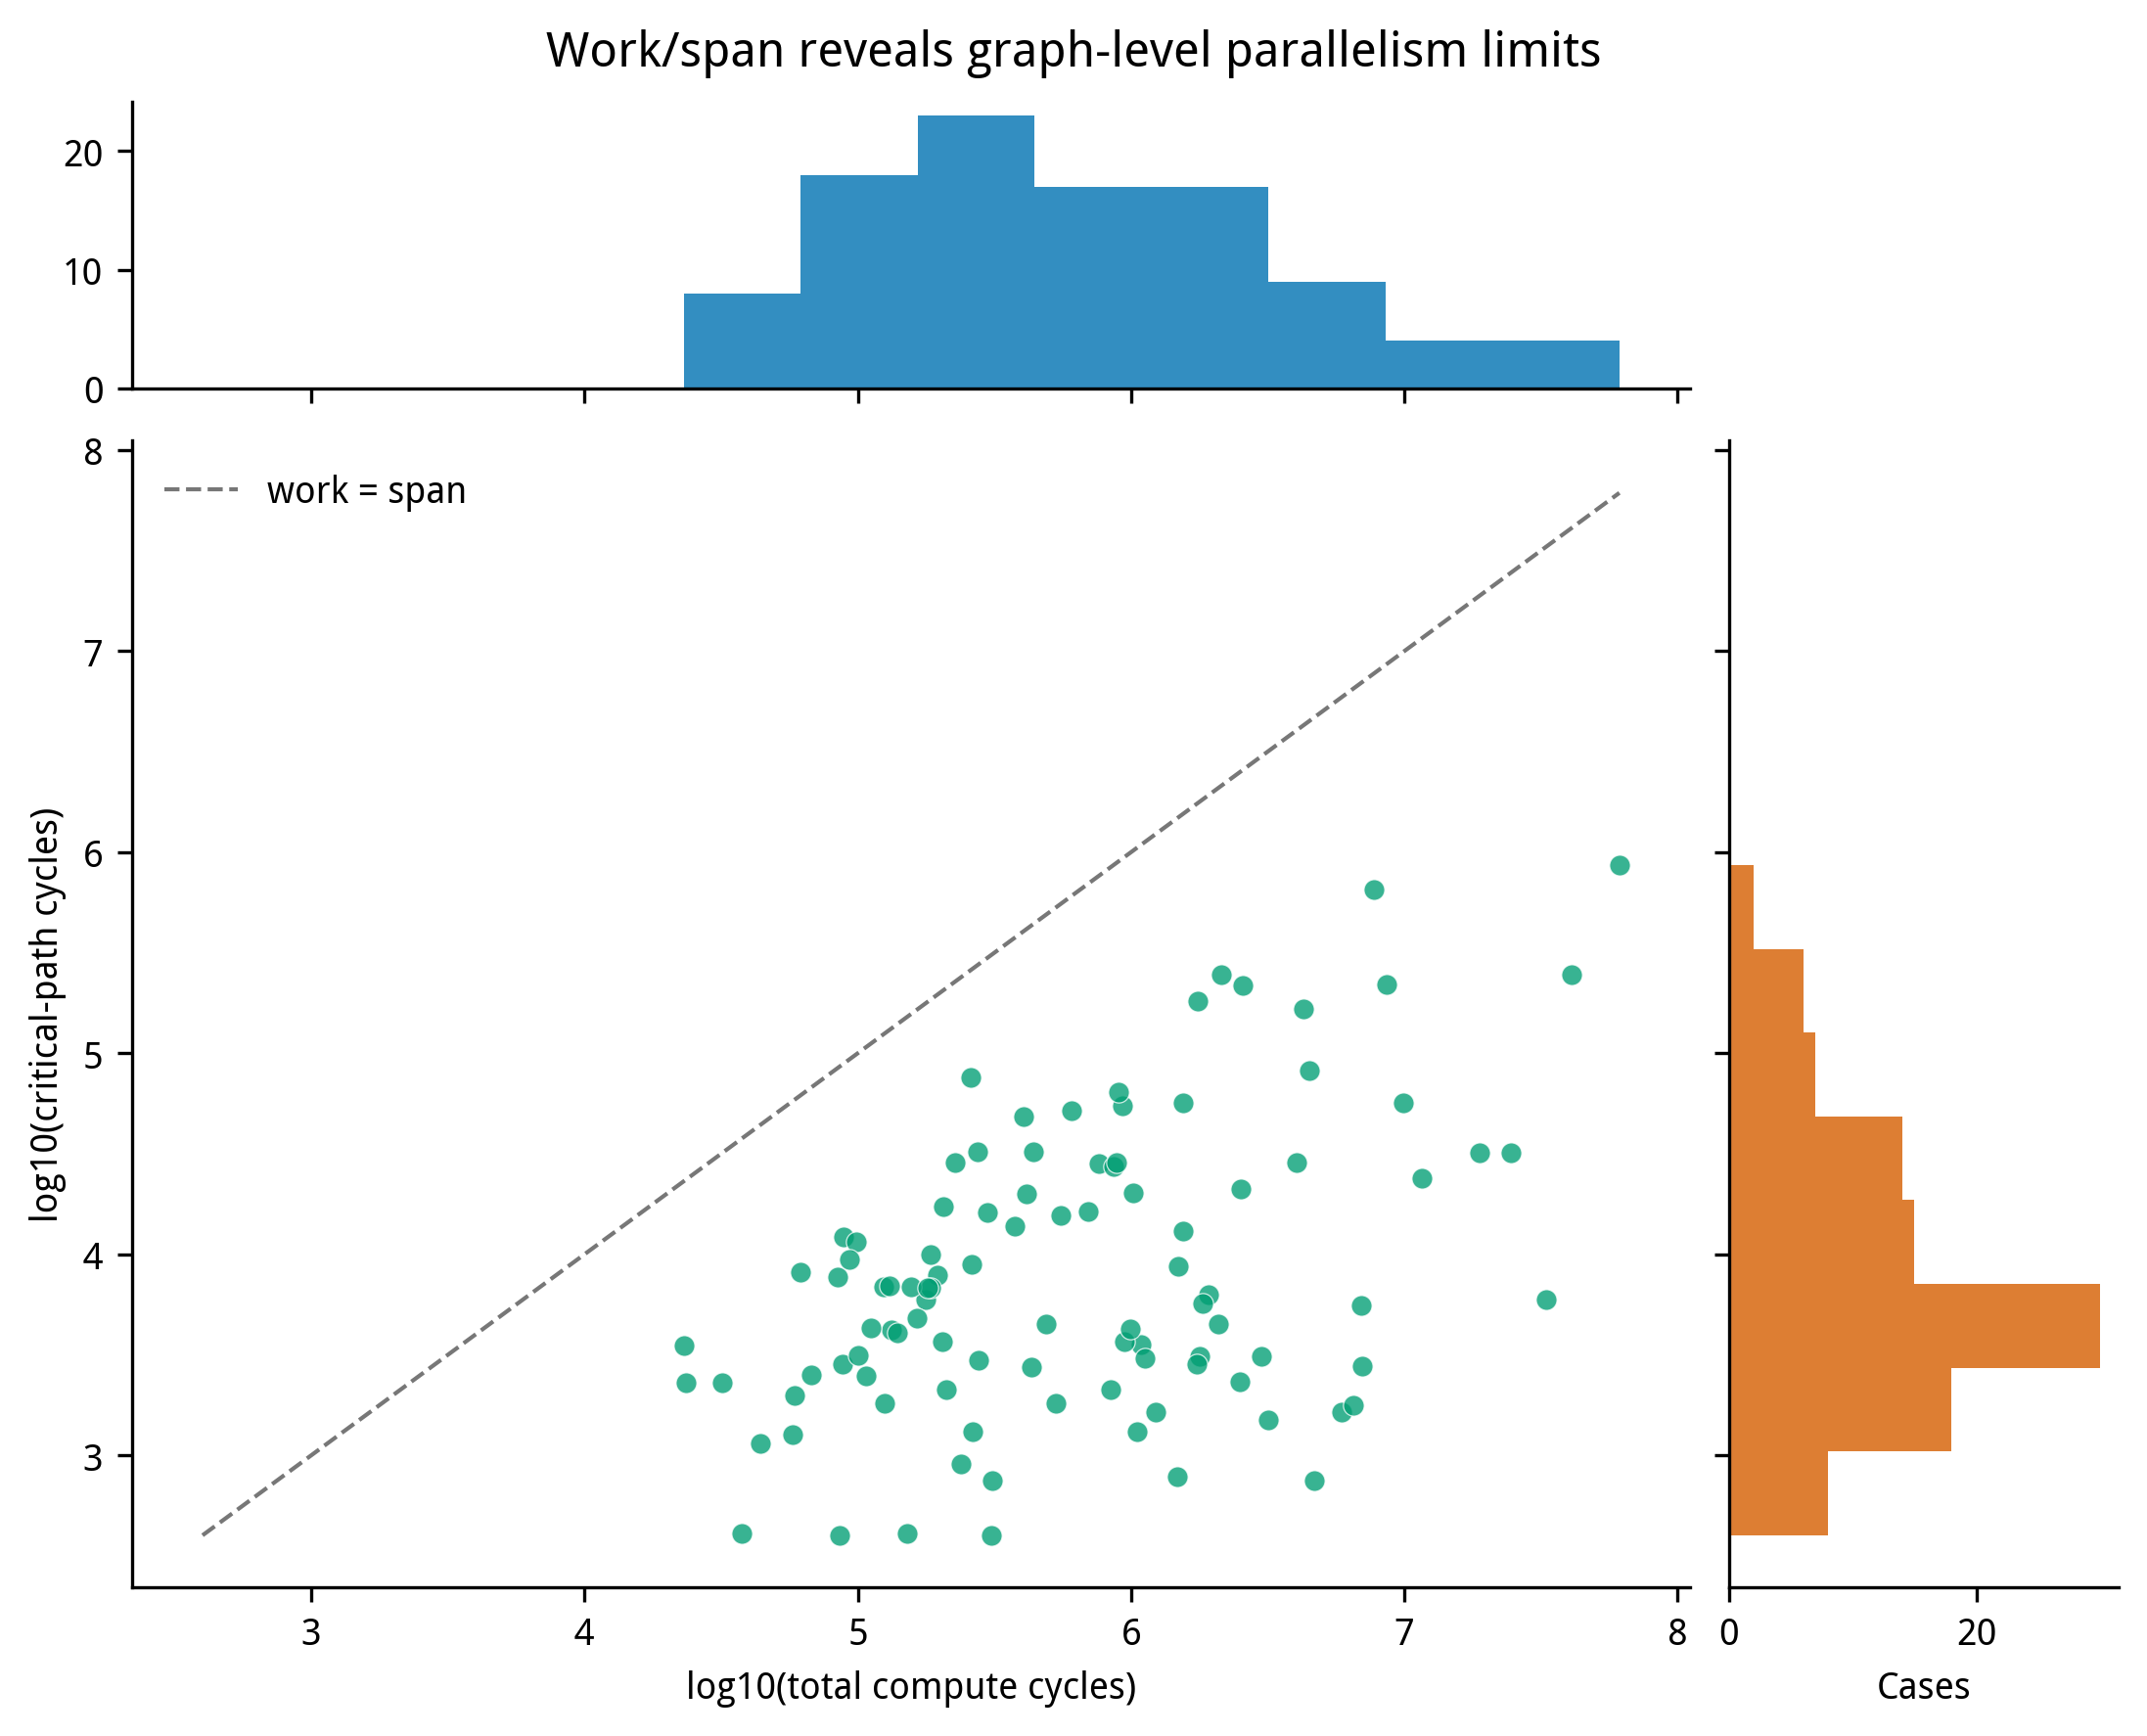
\includegraphics[width=0.88\linewidth]{../all_questions_fresh_v3/figures/fig02_work_span_joint.png}
\caption{总工作量与关键路径的关系}
\end{figure}
\subsection{连通结构、张量与局部性特征}
\begin{center}\textbf{表 5-2  输入图的依赖结构和张量特征}\end{center}
\begin{table}[htbp]
\centering\small
\begin{tabular}{lrrrrrr}
\toprule
特征 & min & Q1 & 中位数 & 均值 & Q3 & max \\
\midrule
弱连通分量数 & 1 & 17.5 & 39.5 & 146.97 & 107.25 & 2,666 \\
最大分量节点占比 & 0.0004 & 0.0156 & 0.1220 & 0.3293 & 0.7288 & 1.0000 \\
张量总数 & 816 & 1,593.25 & 4,590.5 & 7,477.86 & 8,004 & 40,287 \\
张量总字节 & 325,708 & 3,921,341 & 9,366,784 & 29,375,957.16 & 24,141,591 & 360,593,104 \\
外部输入张量数 & 12 & 130 & 254 & 486.68 & 556.5 & 4,362 \\
外部输入字节 & 35,622 & 435,535 & 1,063,082 & 2,083,082.98 & 2,428,224 & 13,400,064 \\
输出张量数 & 1 & 19.5 & 62 & 159.44 & 126.5 & 2,666 \\
输出张量字节 & 2 & 271.5 & 16,689 & 324,217.56 & 160,768 & 4,094,976 \\
\bottomrule
\end{tabular}
\end{table}
100 个案例中有 16 个仅含一个弱连通分量，84 个含多个分量，且这 84 个案例均不少于 5 个分量。最大分量占比的中位数为 12.2\%，上四分位数约为 72.9\%，表明案例间既有分散的小分量，也有单一大分量占主导的图结构，单一分配策略难以覆盖全部情况。

97 个案例至少有一个共享外部输入张量。共享输入可能形成跨核复用机会，也可能因消费者被分配到多个核心而扩大通信。张量总字节均值明显高于中位数，反映不同案例的数据规模差异较大；后续通信和内存分析需同时考察字节数与消费者分布。

\begin{figure}[htbp]
\centering
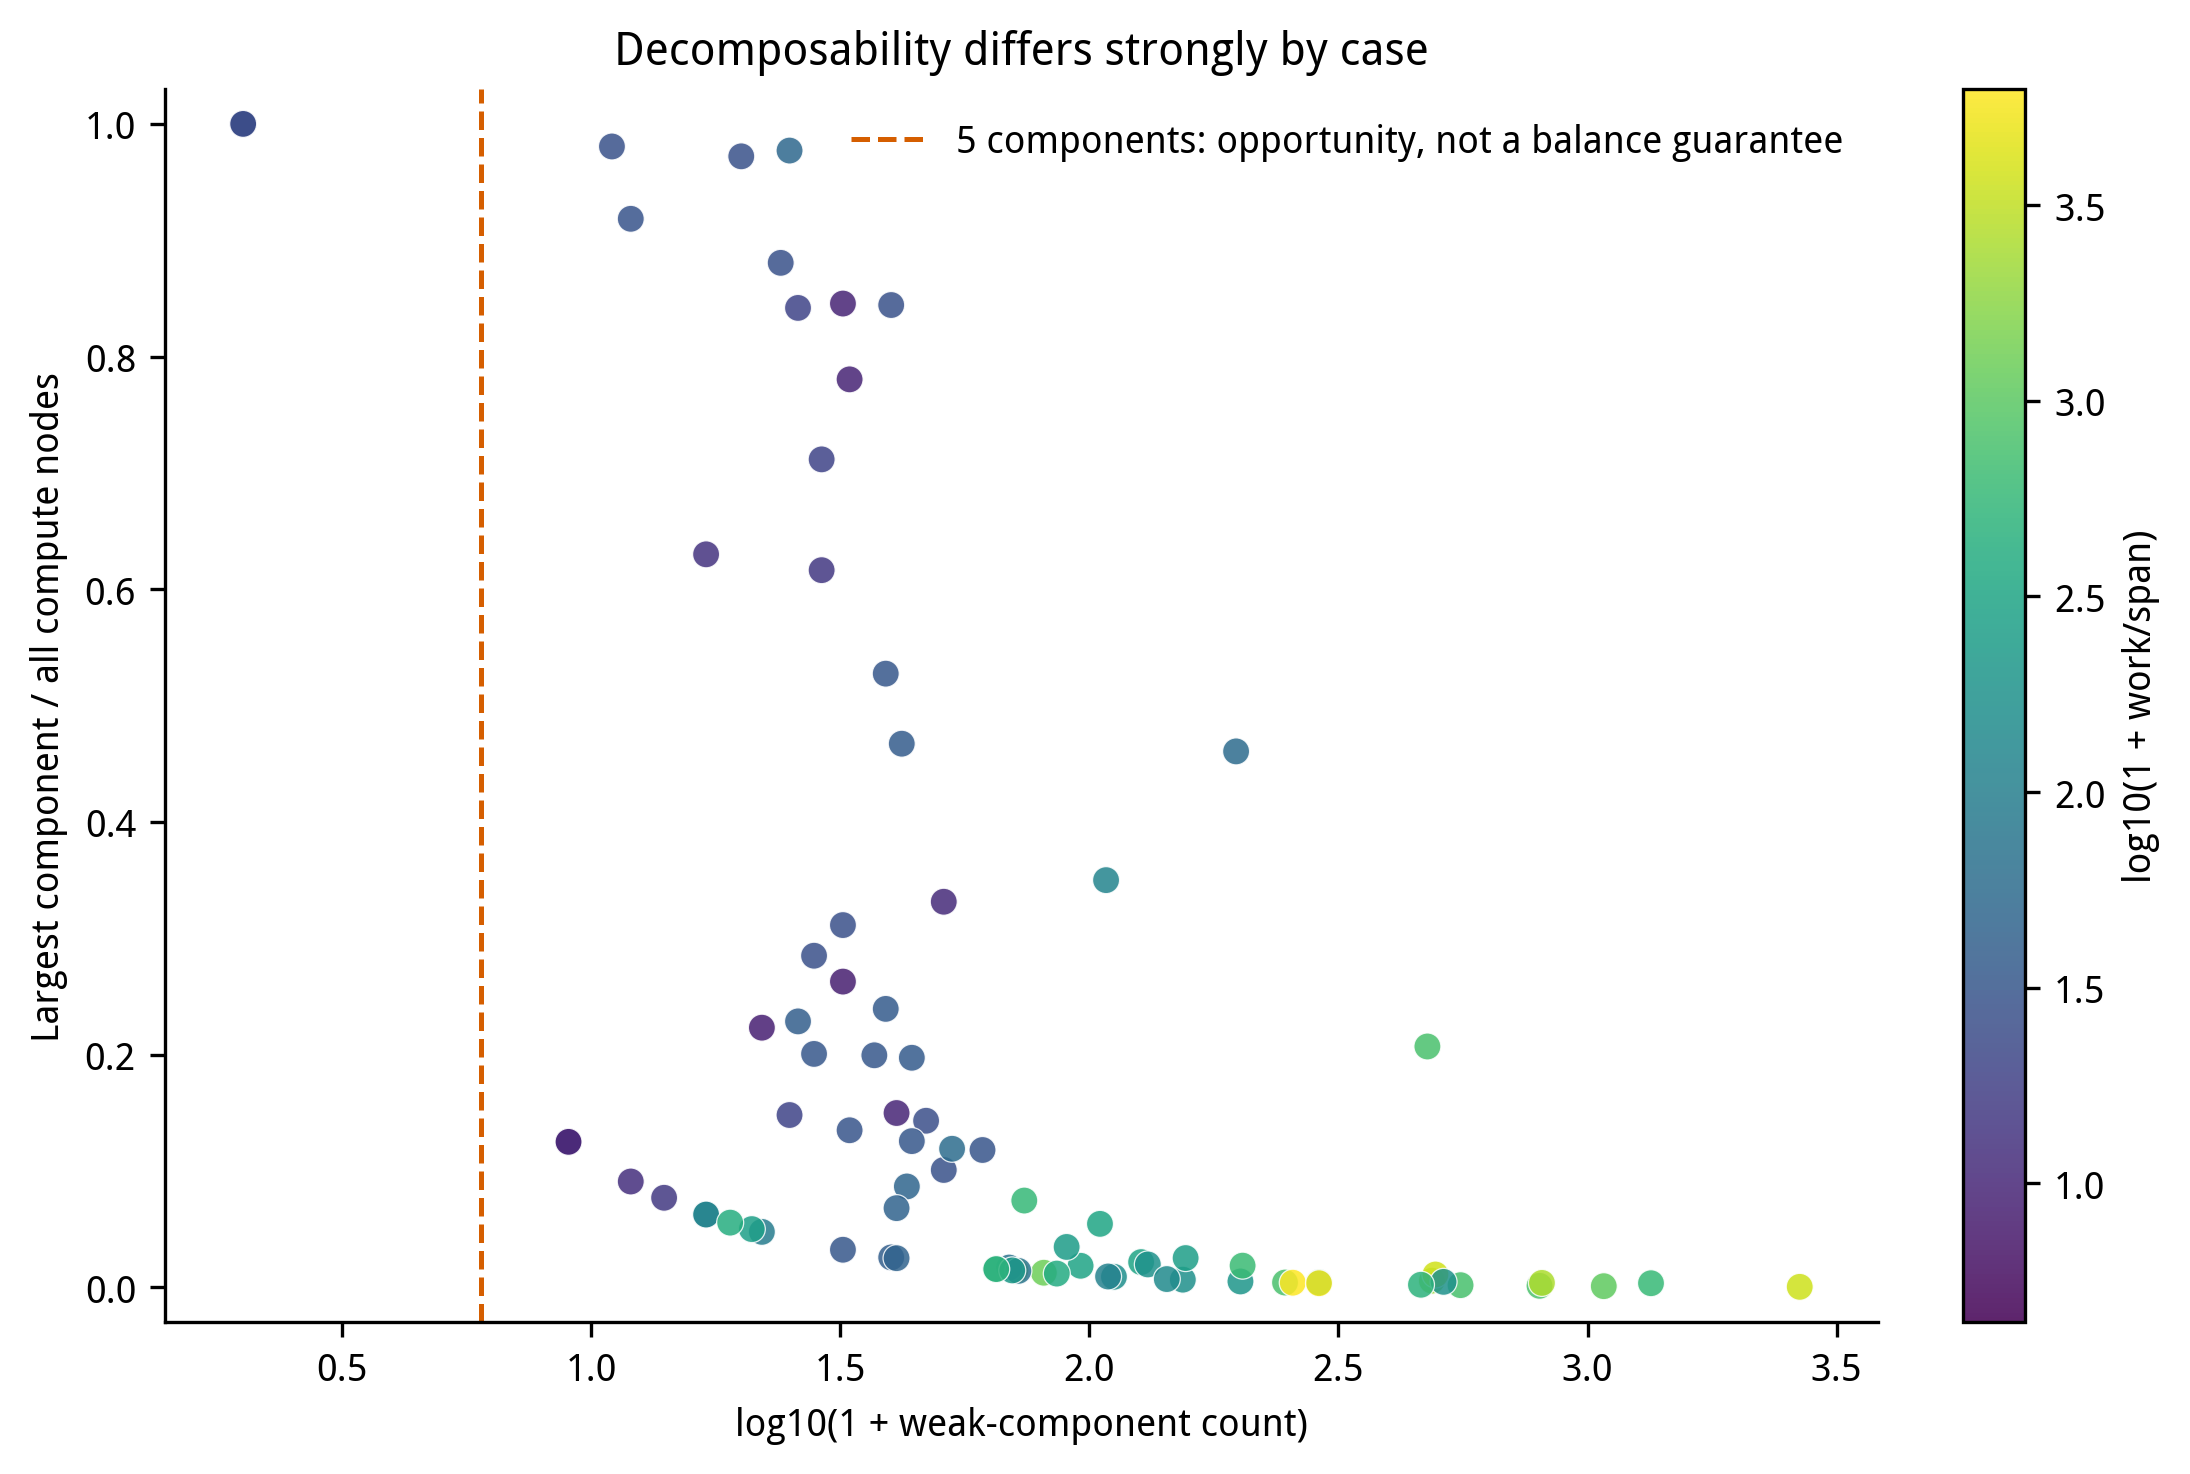
\includegraphics[width=0.88\linewidth]{../all_questions_fresh_v3/figures/fig03_component_structure.png}
\caption{弱连通分量数量及最大分量占比}
\end{figure}
\begin{figure}[htbp]
\centering
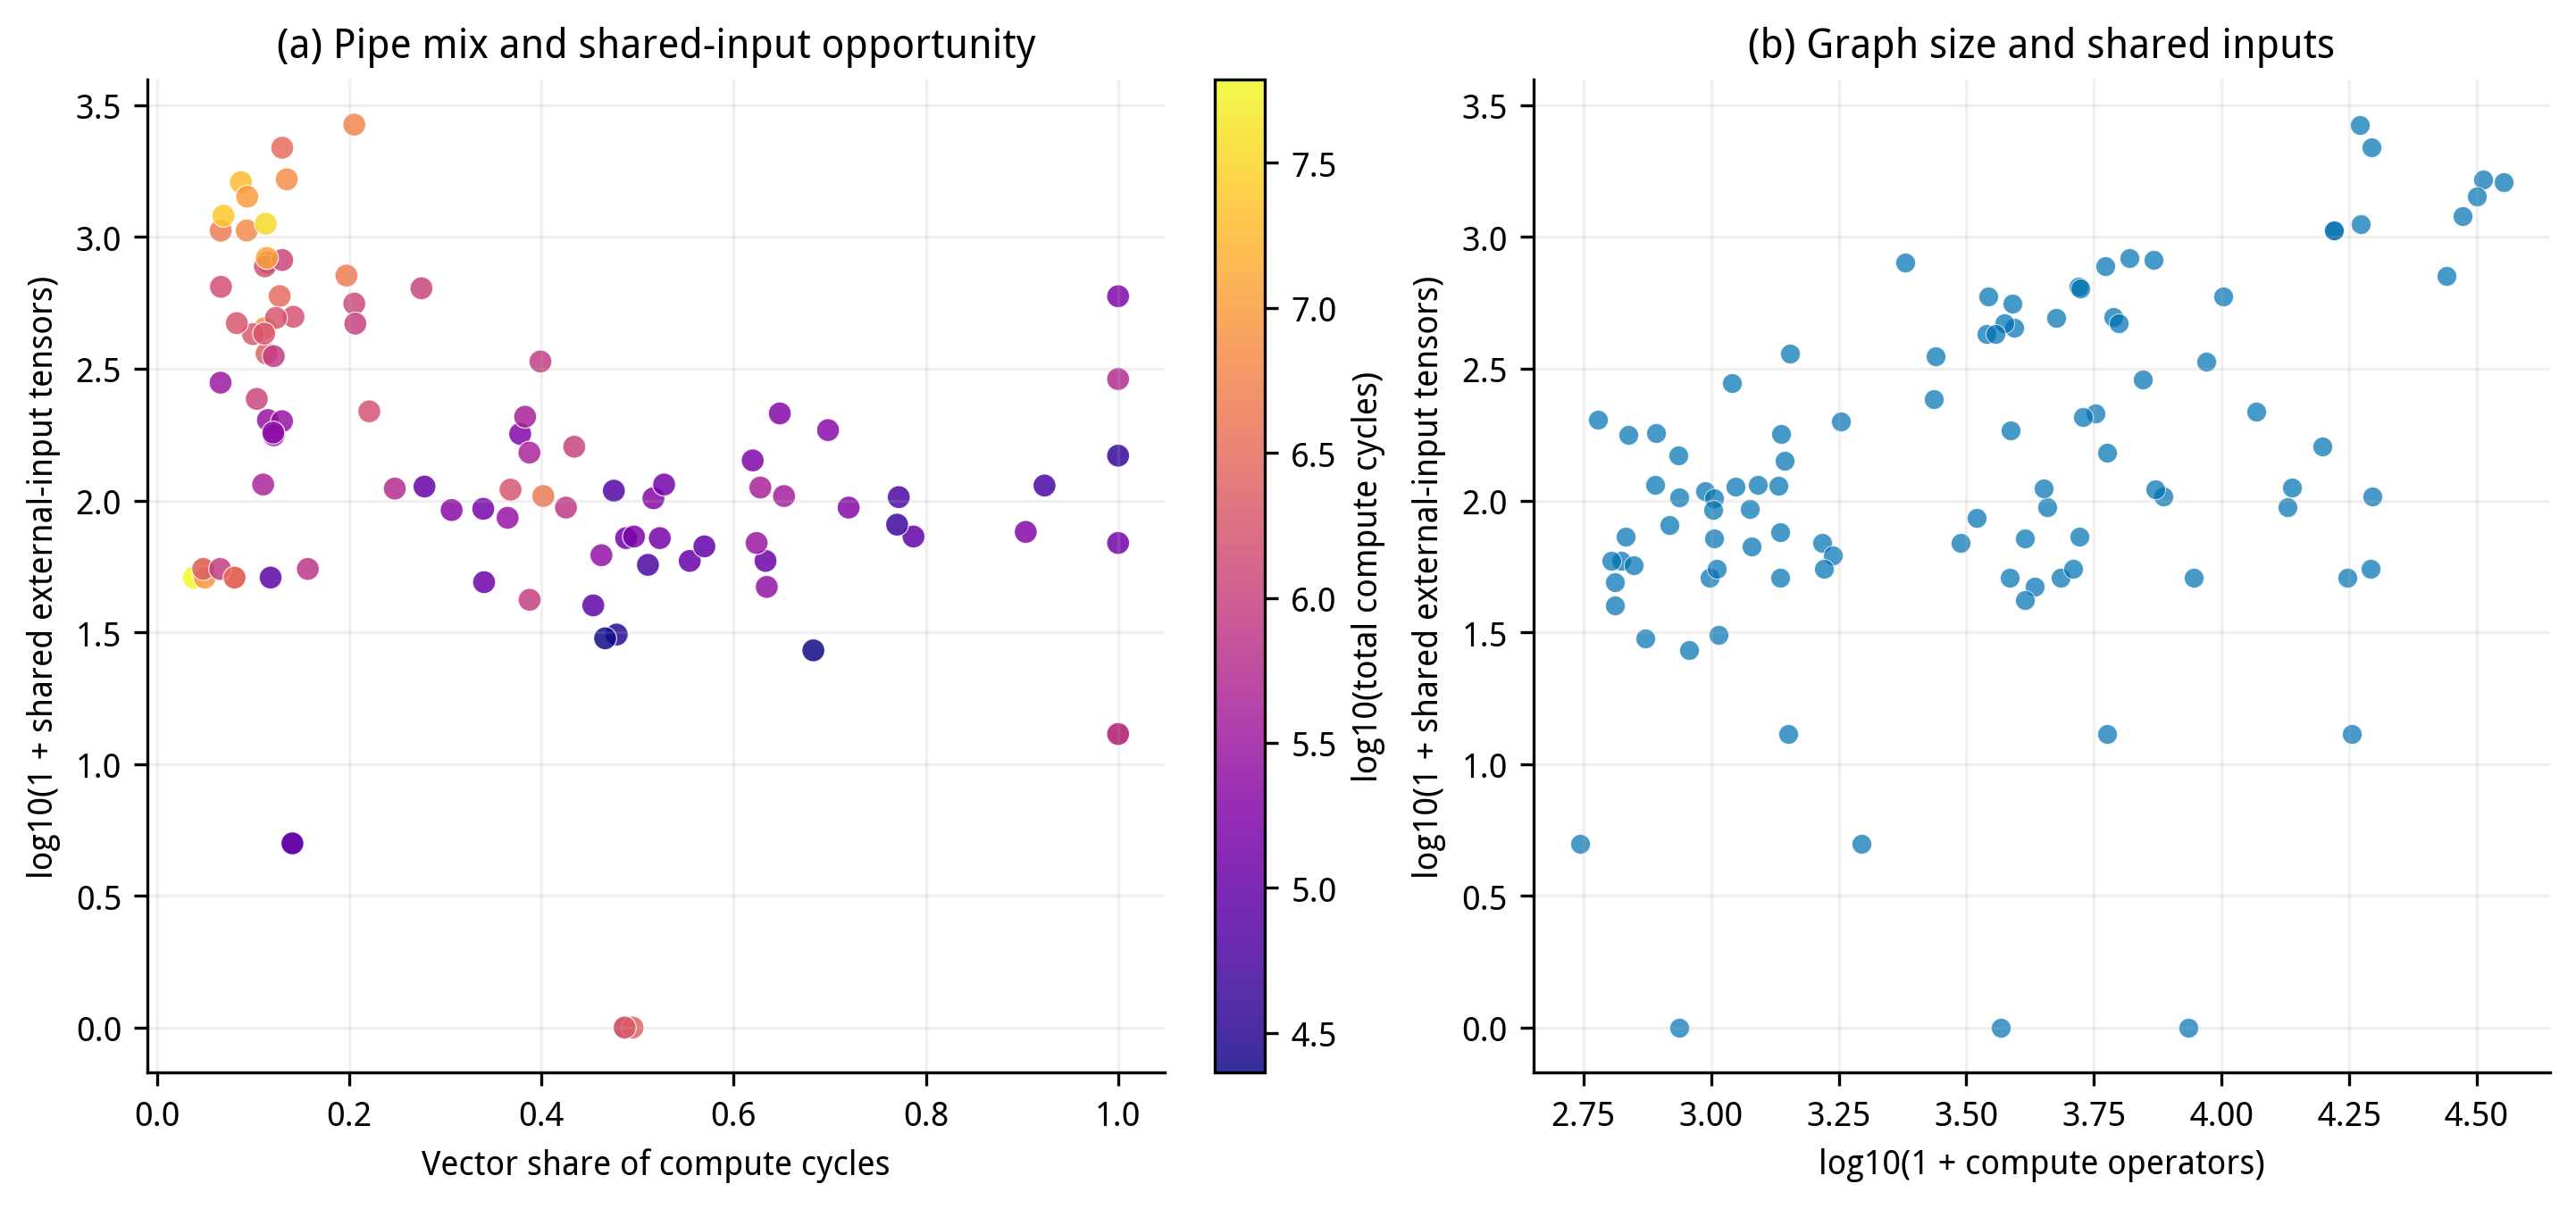
\includegraphics[width=0.88\linewidth]{../all_questions_fresh_v3/figures/fig04_pipe_and_shared_inputs.png}
\caption{矩阵和向量 Pipe 构成及共享输入}
\end{figure}
\subsection{变量相关性和结构分组}
\begin{figure}[htbp]
\centering
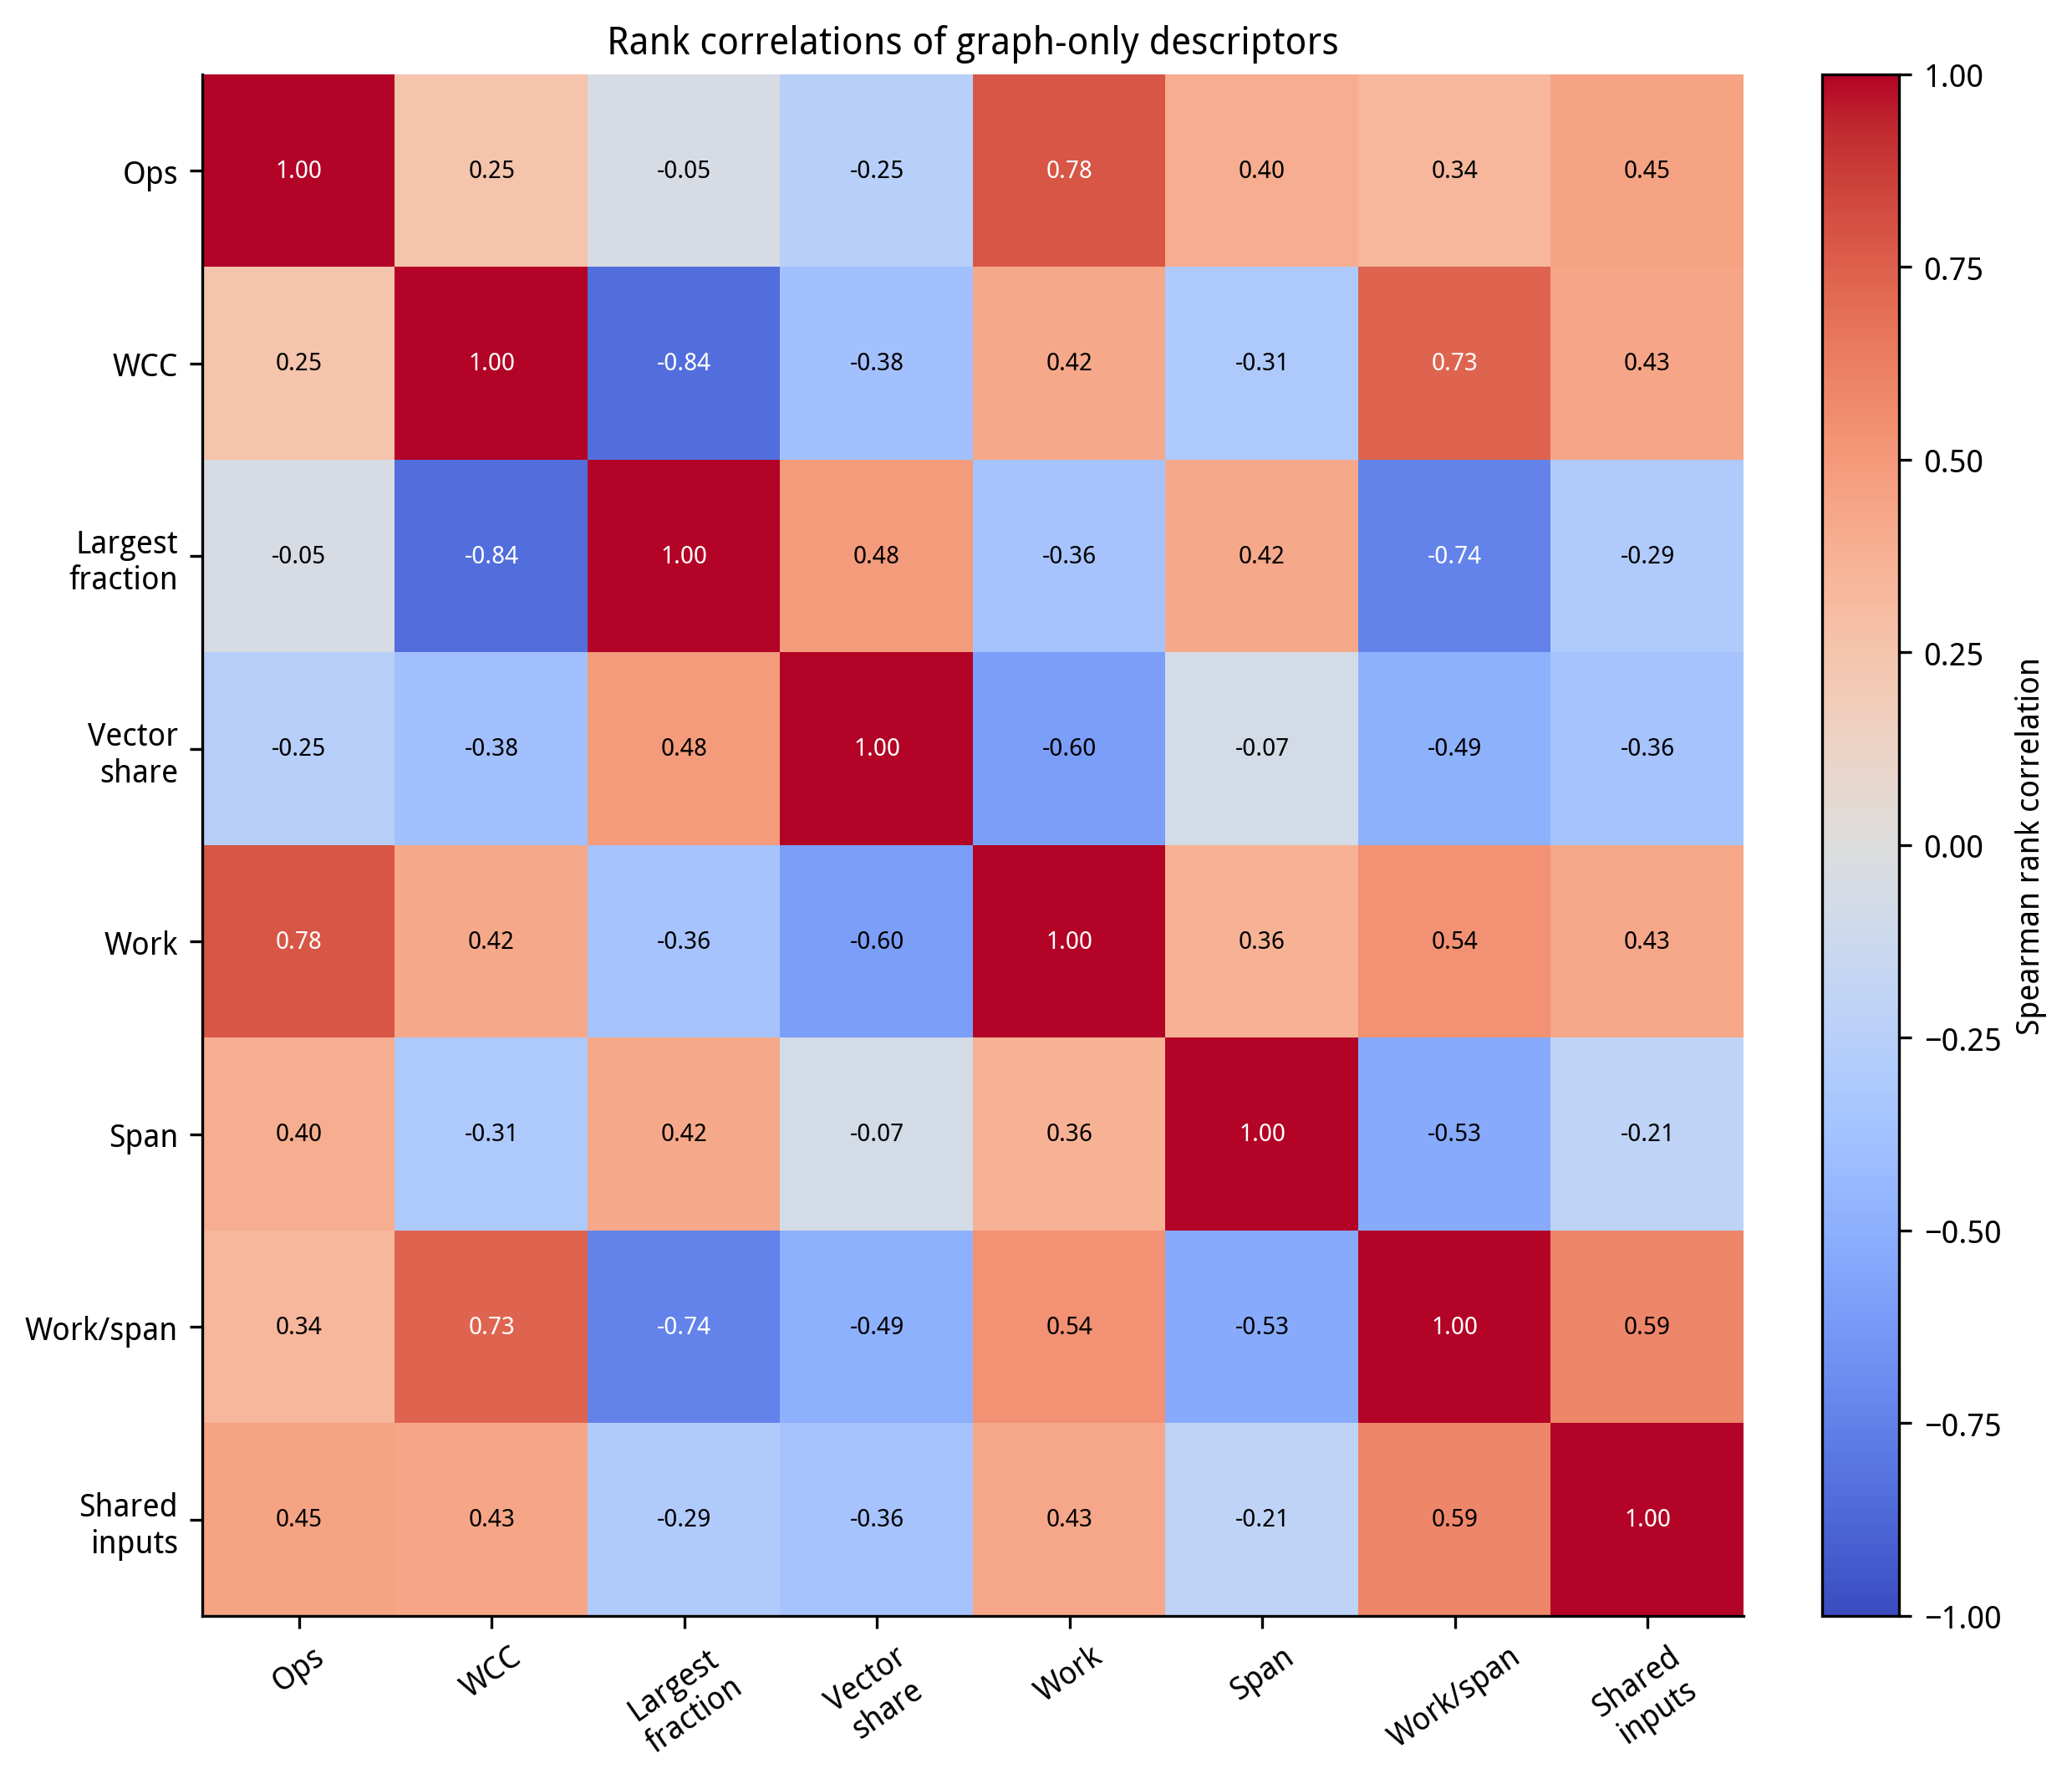
\includegraphics[width=0.88\linewidth]{../all_questions_fresh_v3/figures/fig05_spearman_heatmap.png}
\caption{图规模与计算特征的 Spearman 相关系数}
\end{figure}
\begin{figure}[htbp]
\centering
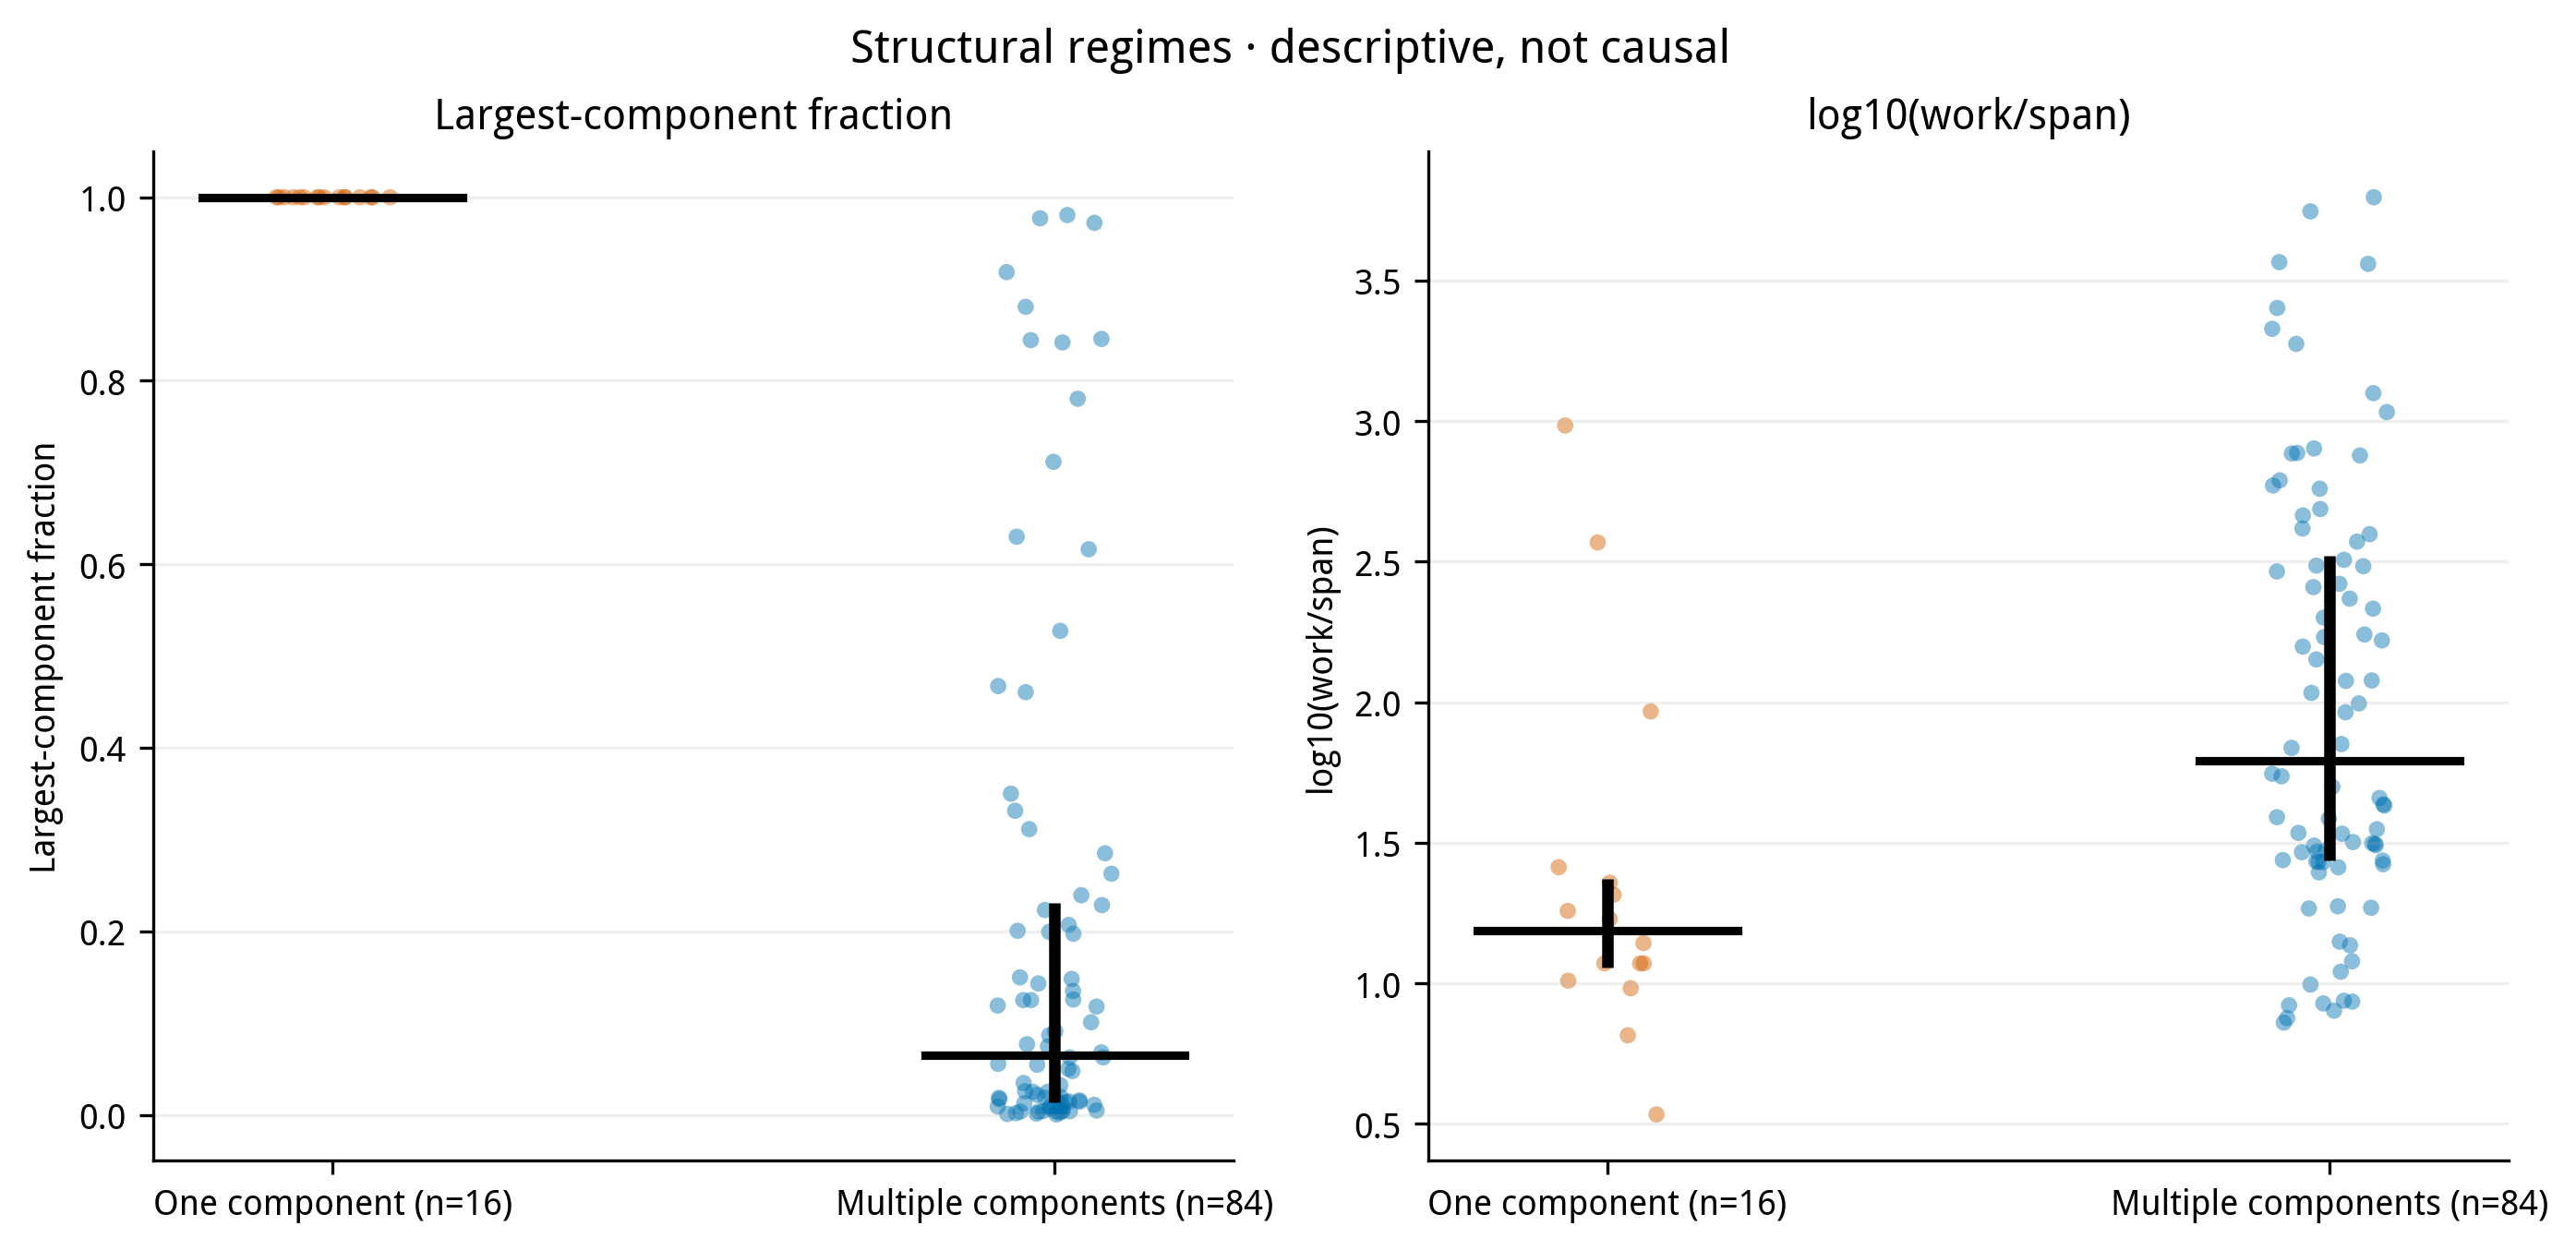
\includegraphics[width=0.88\linewidth]{../all_questions_fresh_v3/figures/fig06_component_regimes.png}
\caption{按分量结构分组的关键特征中位数与四分位范围}
\end{figure}
相关性图用于观察输入特征间的单调关联，不作因果解释。结构分组图以中位数和四分位范围描述组内差异。分量较多不必然意味着更高的并行收益；仍需结合各分量的矩阵/向量工作量、依赖深度和张量边界判断。

\subsection{图结构代理候选及解释范围}
\begin{figure}[htbp]
\centering
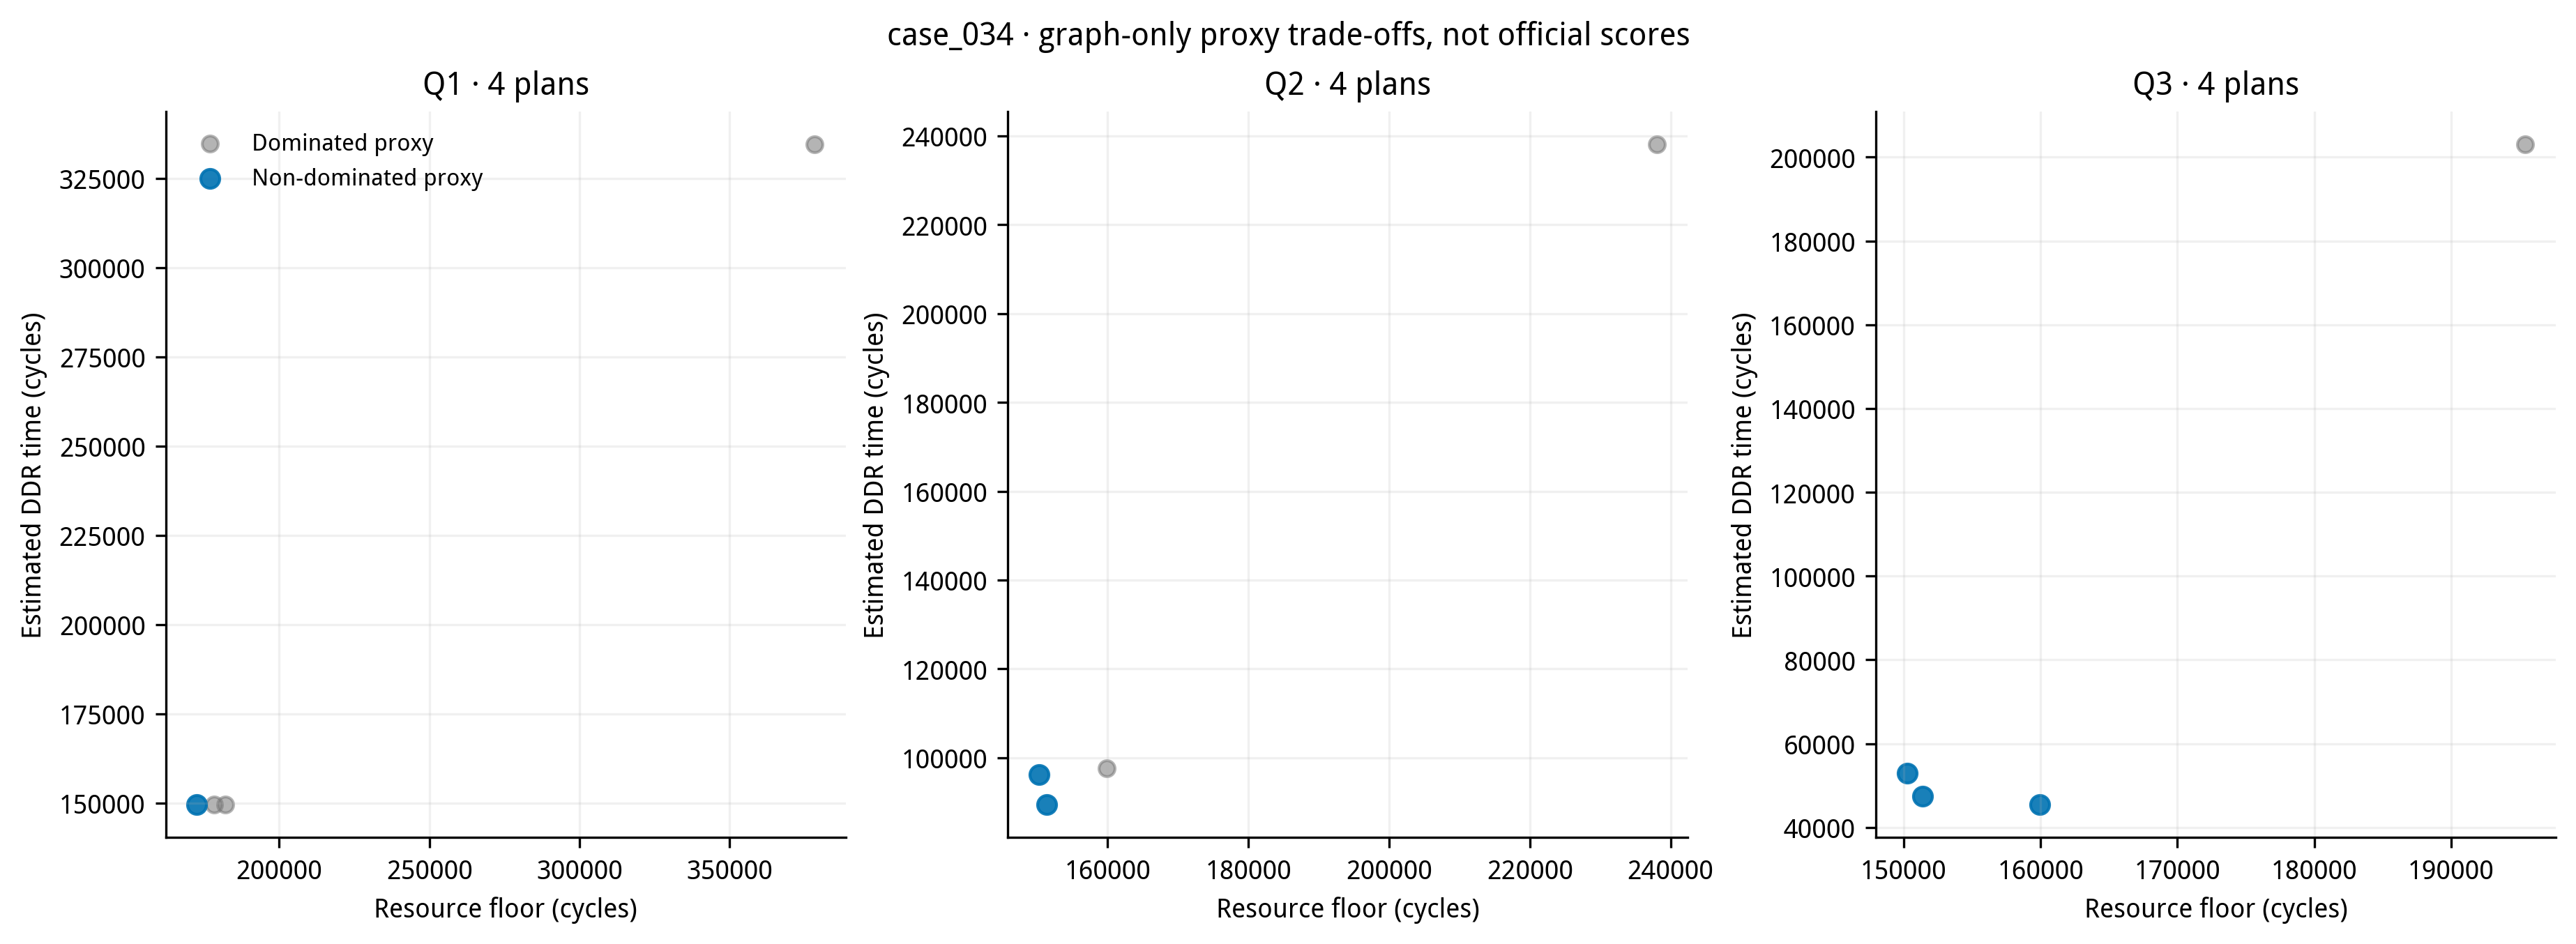
\includegraphics[width=0.88\linewidth]{../all_questions_fresh_v3/figures/fig07_graph_only_pareto.png}
\caption{图结构候选的代理目标 Pareto 对比}
\end{figure}
图 5-7 展示少量结构基线在资源下界、估计通信、逻辑存储超额和 FIFO 代理指标上的权衡。该图不使用官方评估器，不代表真实 makespan 排名、存储可行性证书或 100 个案例的算法性能结果。

\begin{figure}[htbp]
\centering
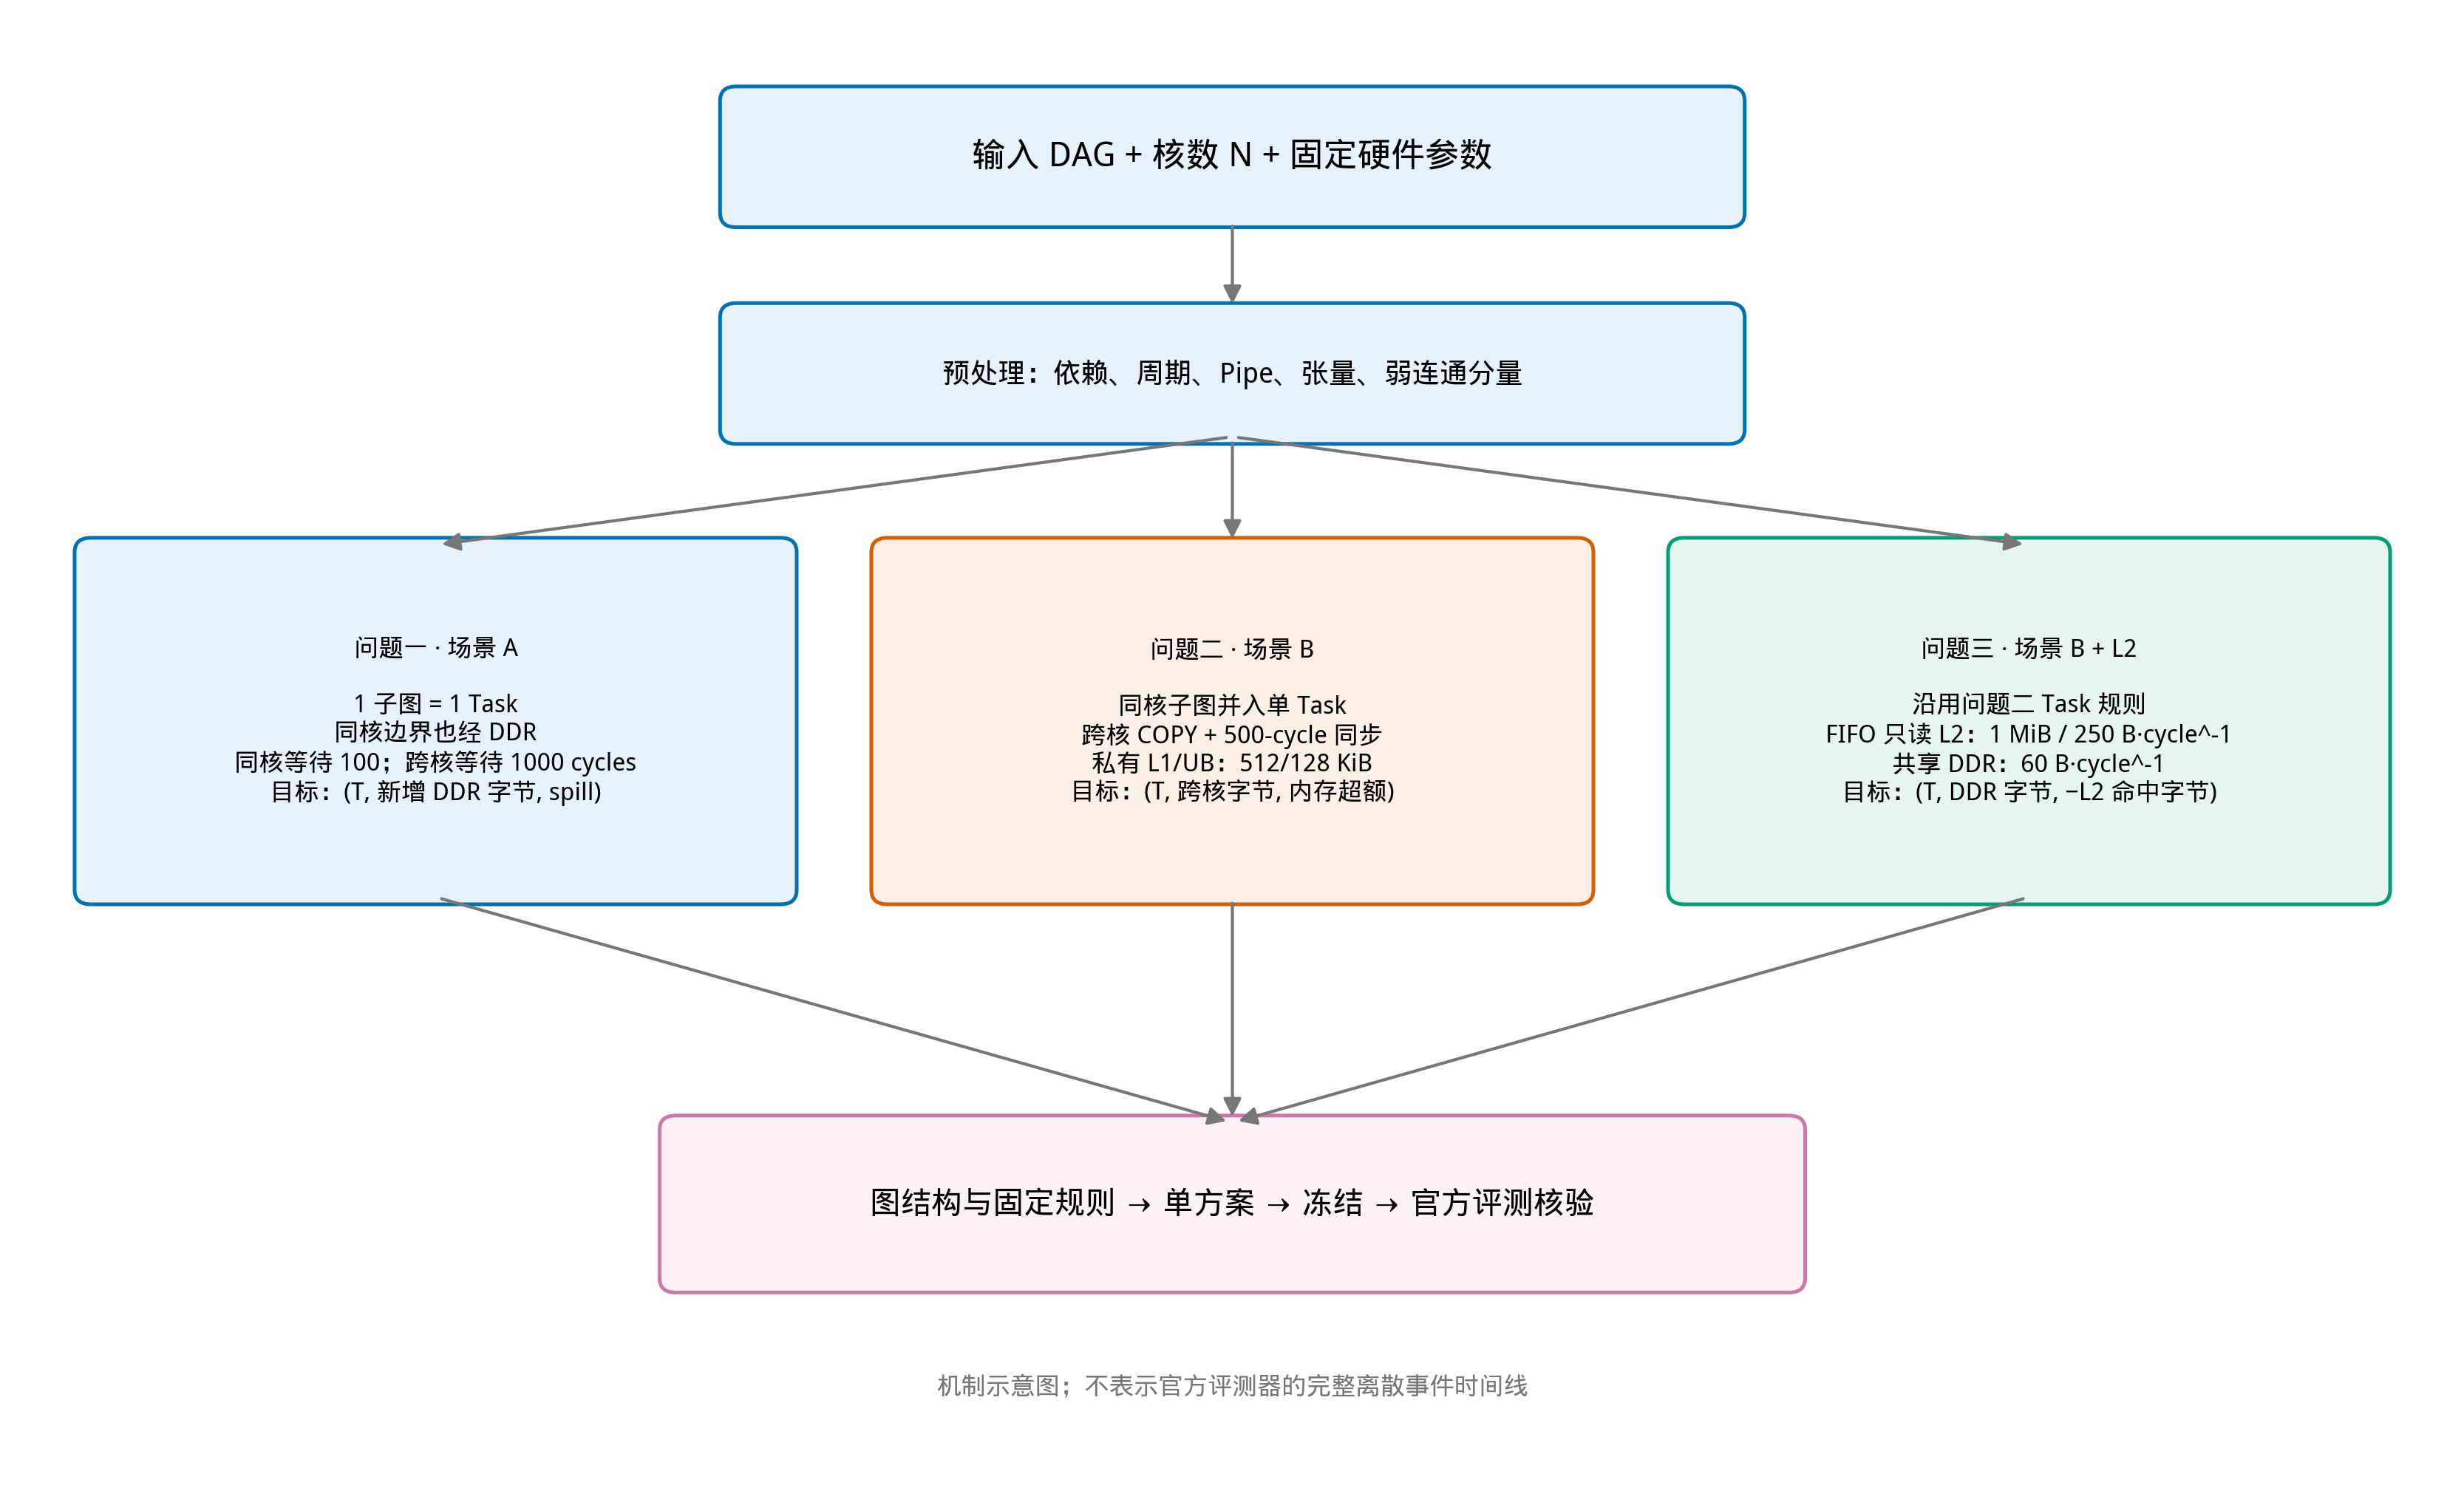
\includegraphics[width=0.88\linewidth]{../all_questions_fresh_v3/figures/fig08_three_scene_model.png}
\caption{三种执行场景的机制差异}
\end{figure}
\section*{参考文献}
\begin{enumerate}[label={[\arabic*]}]
\item 《通用神经网络处理器下的多核切图与协同调度优化模型与算法》，2026 年 A 题第二篇论文，29 页，第 2 章、第 4—6 章及附录 A—C。
\item 2026 年 A 题题目说明及官方输入图、硬件执行配置。具体 Task、COPY、同步、容量和带宽语义以相应版本题面与官方执行程序为准。
\end{enumerate}
\end{document}
